%=== CHAPTER FIVE (5) ===
%=== Discussion ===

\chapter{Experimental Results and Discussion}
\label{cha:experiments}
\begin{spacing}{1.5}
\setlength{\parskip}{0.3in}

\section{Introduction}

This chapter will show the experiment results and the analysis of them.

\autoref{sec:EX_testmetric} will describe the metrics used to evaluate network performance. \autoref{sec:EX_multivisual} will show a tool developed by me to visualize each class in different colour and transparency, and it should be valuable for other researchers to use. \autoref{sec:EX_multiclass} will give the experimental results of RVPGNet by accuracy and loss. It achieves as high as $97.19\%$ multi-class accuracy. \autoref{sec:EX_rainy} will show that the network's performance in rainy conditions is stable, as good as $99.73\%$ $F_1$ score results. \autoref{sec:EX_threshold} will show how to select the output's confidential threshold.

\section{Test Metrics}
\label{sec:EX_testmetric}

We use $F_1$ Score and Accuracy as the test metrics.

Accuracy is given in \autoref{eq:acc}. The symbols in the equation means: TP for true positive, which is correctly predicted positive pixel number; TN for true negative, which is correctly predicted negative pixel number; FP for false positive, which is the number of positive pixels being predicted as negative; FN for false negative, which is the number of negative pixels being predicted as positive. \autoref{fig:testtp} gives clearer interpretation.

\begin{equation}
\label{eq:acc}
    Accuracy=\frac{TP+TN}{TP+TN+FP+FN}=\frac{TP+TN}{All}
\end{equation}

\begin{figure}[ht]
\centering
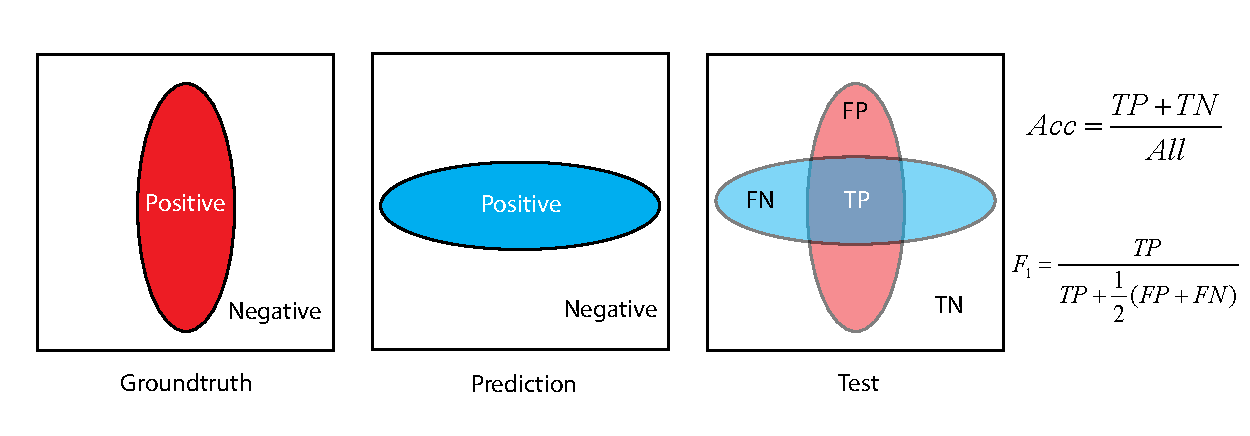
\includegraphics[width=0.99\textwidth, fbox]{Chapter5/testtp.pdf}
\caption{TP, TN, FP and FN in Binary Classification}
\label{fig:testtp} 
\end{figure}

The standard $F_1$ score is given in \autoref{eq:f1score}. It can be presented as a function of recall (\autoref{eq:precision}) and precision (\autoref{eq:recall}), as shown in \autoref{eq:f1pr}:

\begin{alignat}{2}
    Precision &= \frac{TP}{TP+FP} \label{eq:precision}\\
    Recall &= \frac{TP}{TP+FN} \label{eq:recall}\\
    F_1 &= 2\cdot \frac{Precision \cdot Recall}{Precision + Recall} \label{eq:f1pr}\\
     &=\frac{TP}{TP+\frac{1}{2}(FP+FN)} \label{eq:f1score}
\end{alignat}

Especially when there's no positive pixel in the ground truth, and the predicted feature map are all-negative, the $F_1$ score calculated by \autoref{eq:f1score} is zero. However, in this case, all the pixels are predicted precisely. So the $F_1$ score is setted as $1$ in this particular case.

Besides, the RVPGNet uses the metric described in Section 5.3 of VPGNet~\cite{lee2017vpgnet} to calculate the $F_1$ score: 1) calculate the minimum distance between grids' centre and sampled lane points. 2) If the minimum distance is smaller than a boundary value $R$, the sampled lane points are marked as positive. This complies with the output size and the $(8 \times 8)$ grid size in VPGNet. The python code of $F_1$ score calculation are given in \autoref{apx:testmetrics}.

\section{Multi-class Visualization Tool}
\label{sec:EX_multivisual}

\begin{figure}[htbp]
    \centering
    \begin{subfigure}[b]{0.49\textwidth}
        \centering
        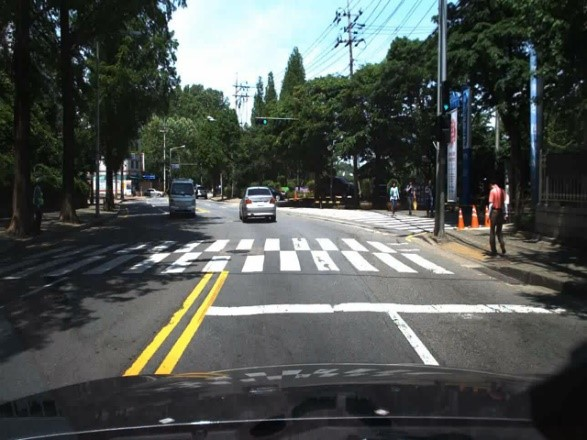
\includegraphics[width=2.7in, fbox]{Chapter5/Picture1.jpg}
        \caption{Picture 1}
    \end{subfigure}%
    ~
    \begin{subfigure}[b]{0.49\textwidth}
        \centering
        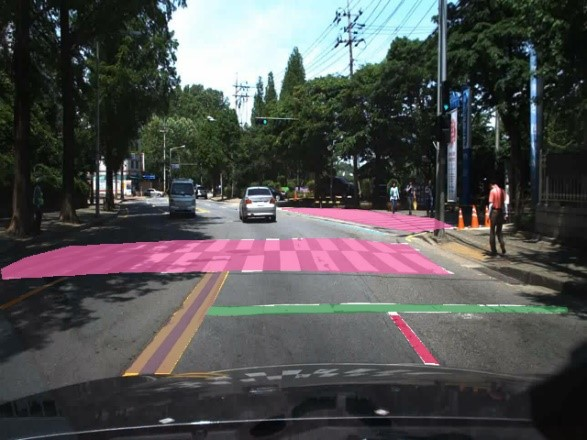
\includegraphics[width=2.7in, fbox]{Chapter5/Picture1an.jpg}
        \caption{Annotated Picture 1, $\alpha$=0.6}
    \end{subfigure}
    \\
    \begin{subfigure}[b]{0.49\textwidth}
        \centering
        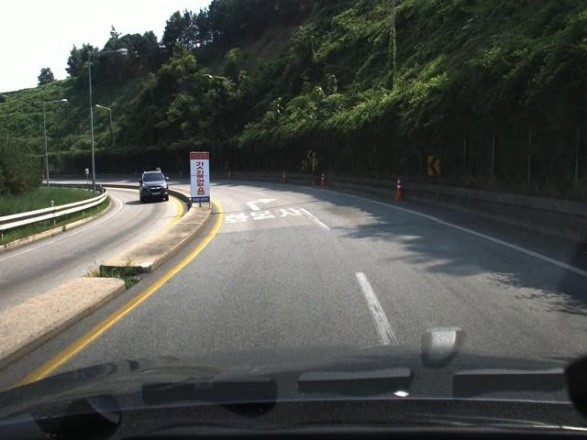
\includegraphics[width=2.7in, fbox]{Chapter5/Picture2.jpg}
        \caption{Picture 2}
    \end{subfigure}%
    ~
    \begin{subfigure}[b]{0.49\textwidth}
        \centering
        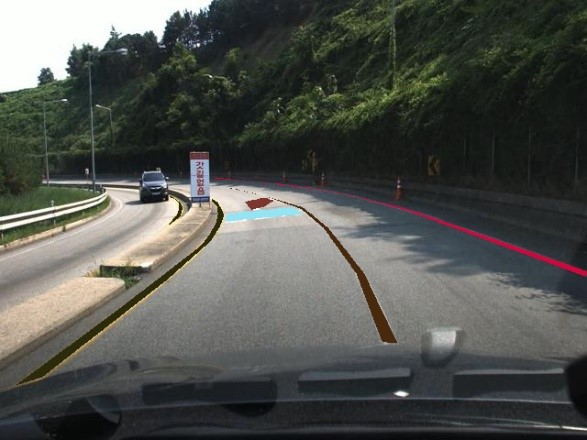
\includegraphics[width=2.7in, fbox]{Chapter5/Picture2an.jpg}
        \caption{Annotated Picture 2, $\alpha=0.8$}
    \end{subfigure}
    \\
    \begin{subfigure}[b]{0.49\textwidth}
        \centering
        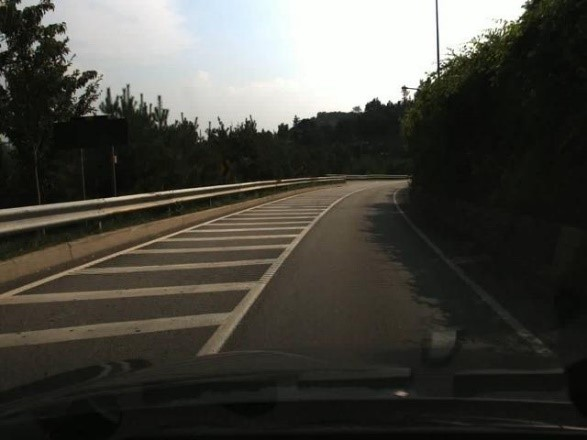
\includegraphics[width=2.7in, fbox]{Chapter5/Picture3.jpg}
        \caption{Picture 3}
    \end{subfigure}%
    ~
    \begin{subfigure}[b]{0.49\textwidth}
        \centering
        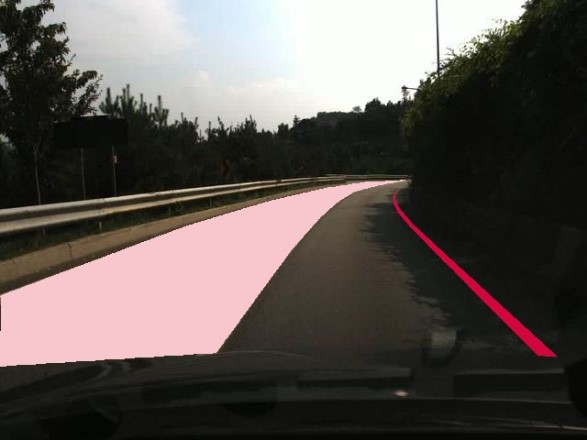
\includegraphics[width=2.7in, fbox]{Chapter5/Picture3an.jpg}
        \caption{Annotated Picture 3, $\alpha=1$}
    \end{subfigure}
    \caption{Multi-class Visualization}
    \label{fig:annotation}
\end{figure}


In this dissertation, an automatic annotation tool was developed to visualize the lane detection result. It can show different classes in a different colour. As shown in \autoref{fig:annotation}, different classes are given colours that are easy to distinguish from each other, and the transparency of the annotation label can be adjusted by a factor $\alpha$. Researchers can also use this tool in other multi-label classification tasks, so the code is included in \autoref{apx:extraction}.

\newpage

\section{Multi-class Performance}
\label{sec:EX_multiclass}

\begin{figure}[ht]
    \centering
    \begin{subfigure}[b]{0.99\textwidth}
        \centering
        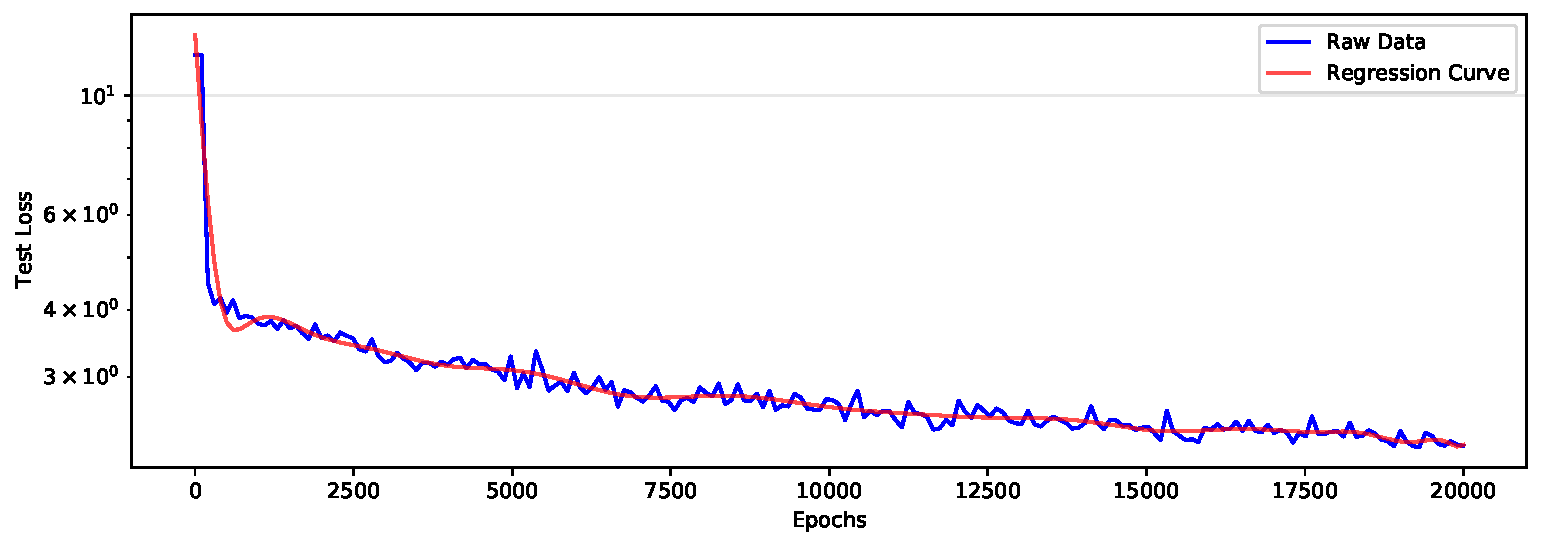
\includegraphics[width=0.98\textwidth, fbox]{Chapter5/testloss20000.pdf}
        \caption{Loss of $20,000$ iteration}
    \end{subfigure}
    \\
    \begin{subfigure}[b]{0.99\textwidth}
        \centering
        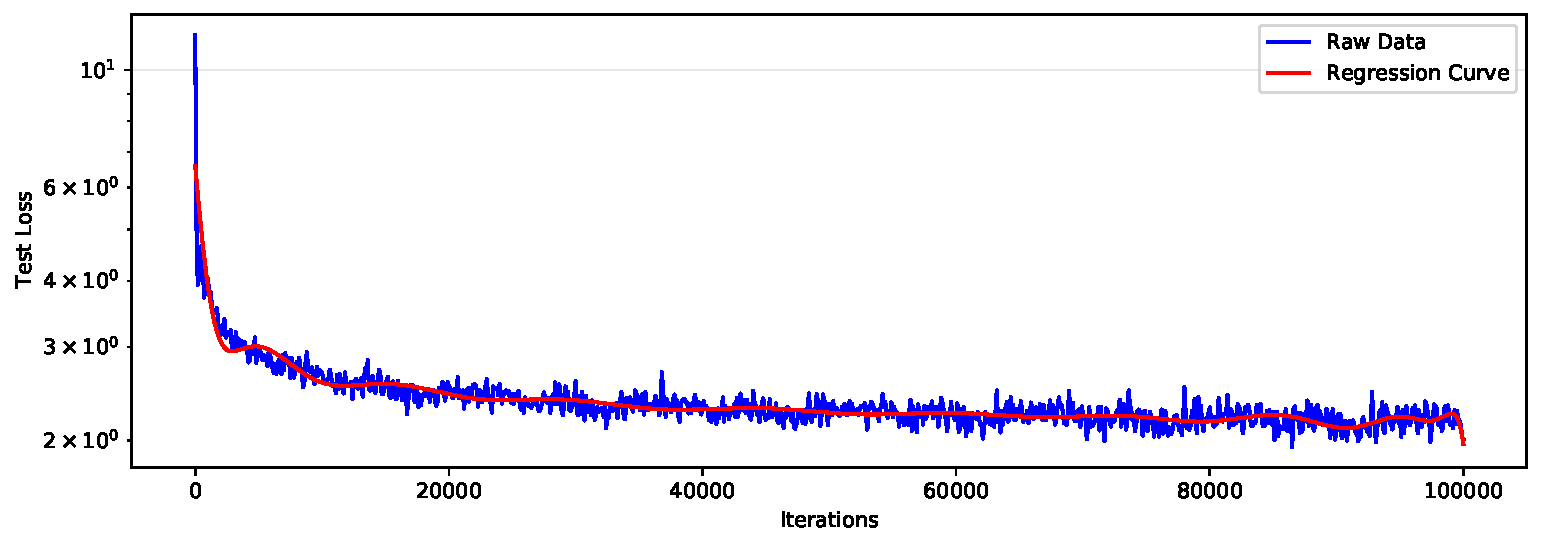
\includegraphics[width=0.98\textwidth, fbox]{Chapter5/testloss100000.pdf}
        \caption{Loss of $100,000$ iteration}
    \end{subfigure}
    \caption{Loss of Training iterations in Caffe}
    \label{fig:testloss}
\end{figure}


First, we conducted experiments on Caffe with different iterations. The training result is shown in \autoref{tab:Cafferesult}. The $Acc_{mask}$ is the masking task accuracy, and the $Acc_{class}$ is the multi-label classification accuracy.

\begin{table}[ht]
\centering
\caption{Training Result on Caffe}
\label{tab:Cafferesult}
\begin{tabular}{@{}cccc@{}}
\toprule
\textbf{iterations} & \textbf{Combined Loss} & \textbf{$Acc_{mask}$} & \textbf{$Acc_{class}$} \\ \midrule
1,000 & 3.73851 & 92.1165\% & 91.6981\% \\
10,000 & 2.7172 & 95.4574\% & 93.5048\% \\
20,000 & 2.53835 & 95.714\% & 93.7822\% \\
40,000 & 2.32726 & 97.37\% & 96.2012\% \\
70,000 & 2.24239 & 97.6137\% & 96.5076\% \\
97,400 & 1.99095 & \textcolor{red}{97.7479\%} & \textcolor{red}{97.1909\%} \\ \bottomrule
\end{tabular}
\end{table}

One way to avoid overfitting is to compare the accuracy in the training and the evaluation process. As shown in \autoref{fig:testloss}, experiment loss with the $20,000$ iterations and $100,000$ iterations are plotted with a regression curve, and Y-axis set as log scale. As can be seen, the loss is decreasing rapidly and converge at around $2.12$. After comparing the training accuracy score with the evaluation accuracy score, we think the network converge at around $100,000$ iterations. If training continues, the over-fitting may happen.

\begin{figure}[ht]
\centering
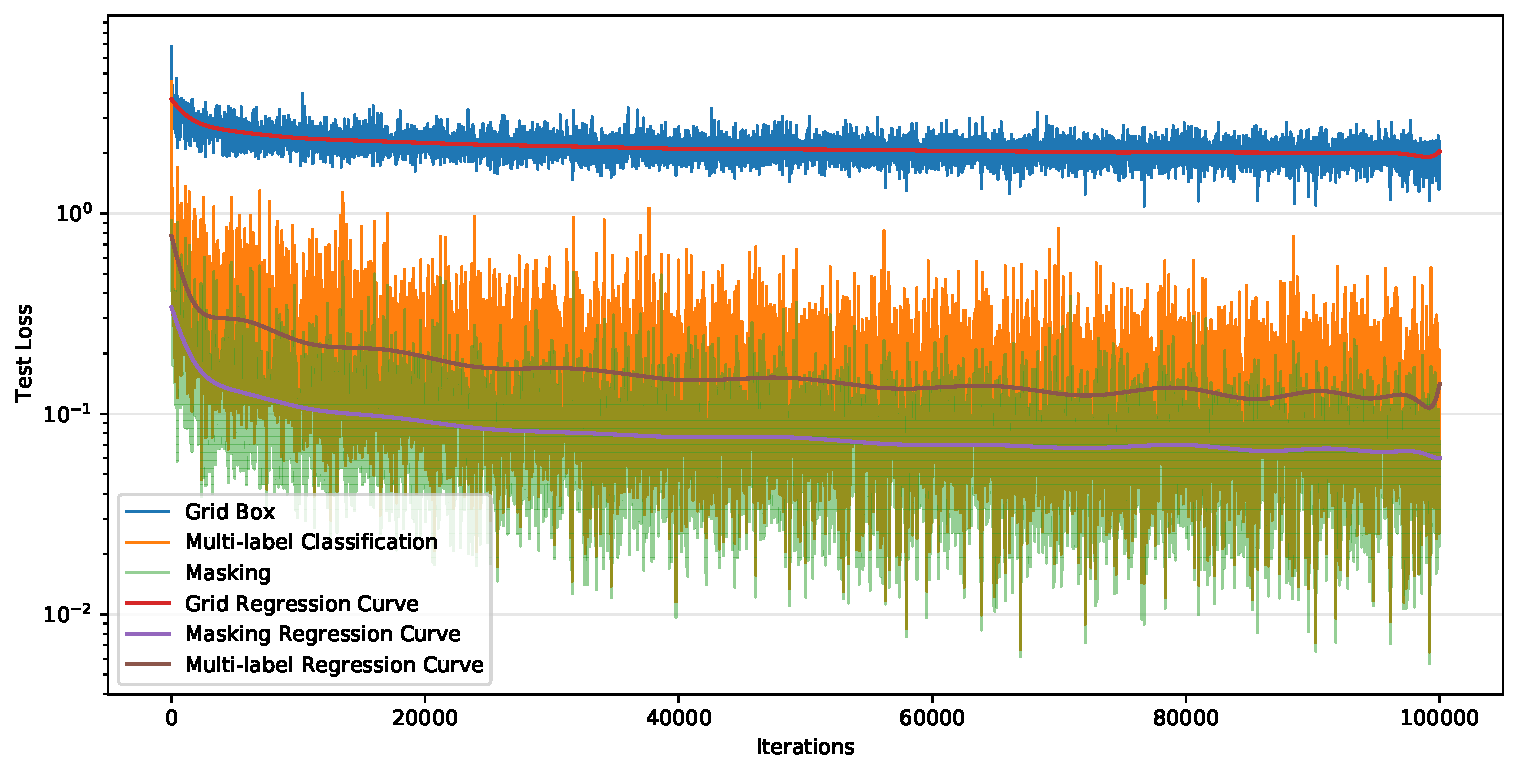
\includegraphics[width=0.99\textwidth, fbox]{Chapter5/testlossbranch.pdf}
\caption{Test Loss in Three Branches Decrease with Different Rate}
\label{fig:testlossbranch} 
\end{figure}

\begin{figure}[ht]
\centering
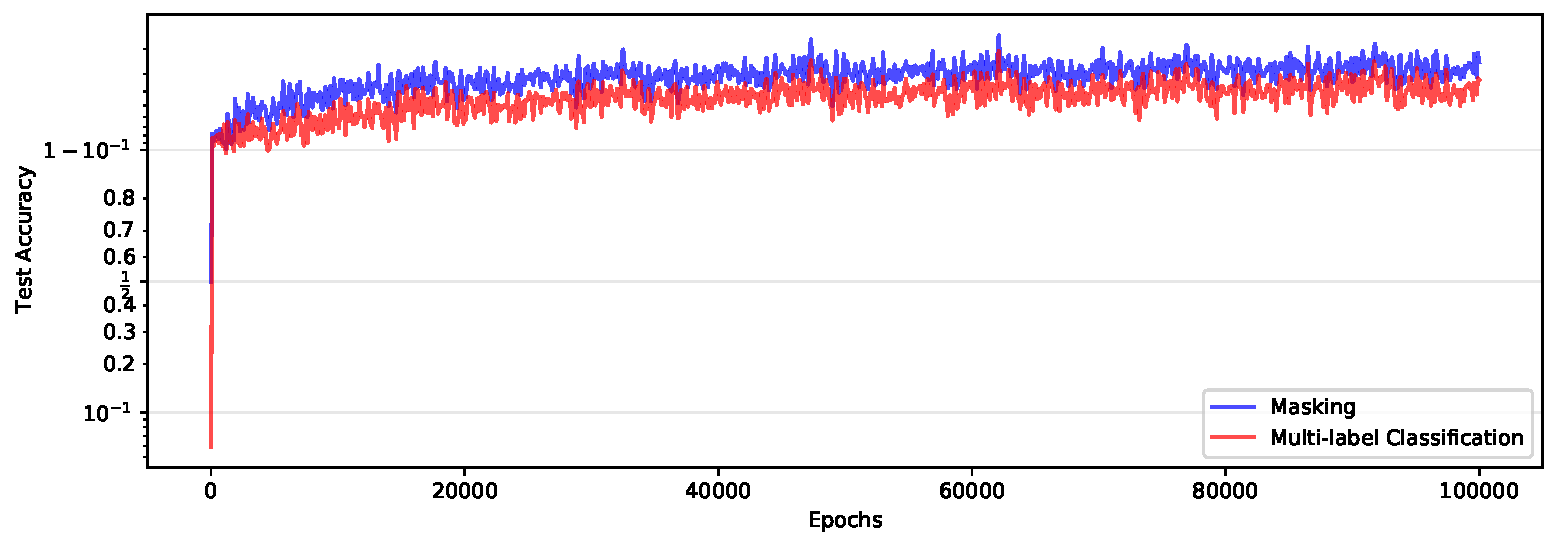
\includegraphics[width=0.99\textwidth, fbox]{Chapter5/testacc.pdf}
\caption{Test Accuracy Curve in Logit Scale $(0,1)$}
\label{fig:testacc} 
\end{figure}


In the experiment, it is found that the loss decreasing rate for different branches is different. As shown in \autoref{fig:testlossbranch}, the grid box's loss is much higher than the other two. As a result, a configuration is employed with $3:1:1$ weight for the grid, the masking and the pixel classification tasks are employed. The combined loss is shown in \autoref{eq:combineloss}.

\begin{equation}
\label{eq:combineloss}
    Loss_{comb}=w_1*{Loss_{grid}}+w_2*{Loss_{masking}}+w_3*{Loss_{cls}}
\end{equation}

in which $w_1=\frac{3}{3+1+1}=0.6$, $w_2=w_3=\frac{1}{3+1+1}=0.2$.


The accuracy curve of the multi-label pixel classification task and masking task are shown in \autoref{fig:testacc}. Notice that because they are close to each other when close to $1$, it uses the Logit scale Y-axis in $(0,1)$.

\section{Rainy Condition}
\label{sec:EX_rainy}

To test the network performance under rainy condition, five samples are picked out. They have very hard-to-recognize features: 

\begin{table}[p]
\centering
\caption{Multi-class $F_1$ Score in Rainy and Bad Illuminance Condition}
\label{tab:rainyf1}
\begin{tabular}{@{}lllllllll@{}}
\toprule
\multicolumn{9}{c}{\texttt{scene\_3/20160809\_1423\_33/000091}} \\ \midrule
1.0 & 0.7743 & 1.0 & 0.8925 & 1.0 & 1.0 & 1.0 & 1.0 & 1.0 \\
1.0 & 1.0 & 1.0 & 1.0 & 1.0 & 1.0 & 1.0 & 0.5074 &  \\
 &  &  &  &  &  &  & Average & 95.14\% \\ \midrule
\multicolumn{9}{c}{\texttt{scene\_3/20160809\_1425\_34/000091}} \\ \midrule
1.0 & 0.6675 & 1.0 & 0.7170 & 1.0 & 1.0 & 1.0 & 1.0 & 1.0 \\
1.0 & 1.0 & 1.0 & 1.0 & 1.0 & 1.0 & 1.0 & 0.4854 &  \\
 &  &  &  &  &  &  & Average & 93.35\% \\ \midrule
\multicolumn{9}{c}{\texttt{scene\_2/20160510\_1302\_22/000181}} \\ \midrule
0.3626 & 1.0 & 1.0 & 1.0 & 1.0 & 1.0 & 1.0 & 1.0 & 0.7151 \\
1.0 & 1.0 & 1.0 & 1.0 & 1.0 & 0.8603 & 1.0 & 1.0 &  \\
 &  &  &  &  &  &  & Average & 93.75\% \\ \midrule
\multicolumn{9}{c}{\texttt{scene\_4/20160518\_2015\_42/000031}} \\ \midrule
0.7362 & 0.4944 & 1.0 & 0.8310 & 1.0 & 1.0 & 1.0 & 1.0 & 1.0 \\
1.0 & 1.0 & 1.0 & 1.0 & 1.0 & 1.0 & 1.0 & 1.0 &  \\
 &  &  &  &  &  &  & Average & 94.48\% \\ \midrule
\multicolumn{9}{c}{\texttt{scene\_4/20160805\_2122\_57/000241}} \\ \midrule
1.0 & 1.0 & 1.0 & 1.0 & 1.0 & 1.0 & 1.0 & 1.0 & 1.0 \\
1.0 & 1.0 & 1.0 & 1.0 & 1.0 & 0.9537 & 1.0 & 1.0 &  \\
 &  &  &  &  &  &  & Average & 99.73\% \\ \bottomrule
\end{tabular}
\end{table}


\begin{figure}[!ht]
    \centering
    \begin{subfigure}[b]{0.49\textwidth}
        \centering
        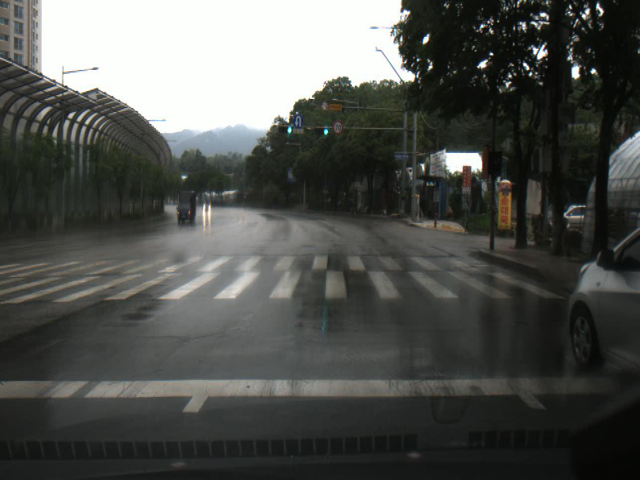
\includegraphics[width=2.7in, fbox]{Chapter5/scene_2-20160510_1302_22-000181.png}
        \caption{Heavy Light Reflection}
        \label{fig:heavylight}
    \end{subfigure}%
    ~
    \begin{subfigure}[b]{0.49\textwidth}
        \centering
        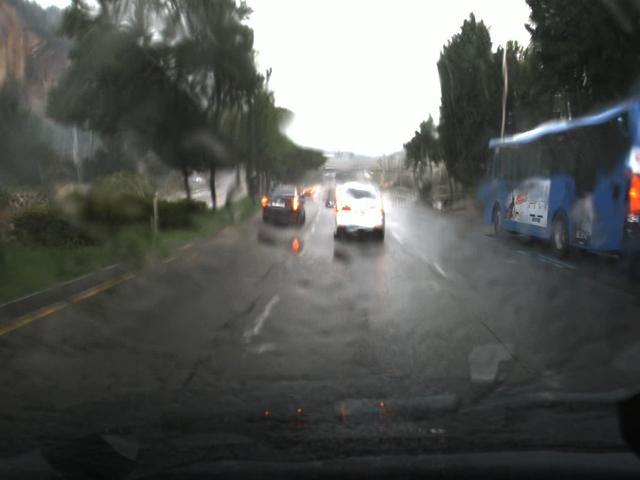
\includegraphics[width=2.7in, fbox]{Chapter5/scene_3-20160809_1423_33-000091.png}
        \caption{Blurred by Rain}
        \label{fig:blurbyrain}
    \end{subfigure}
    \\
    \begin{subfigure}[b]{0.49\textwidth}
        \centering
        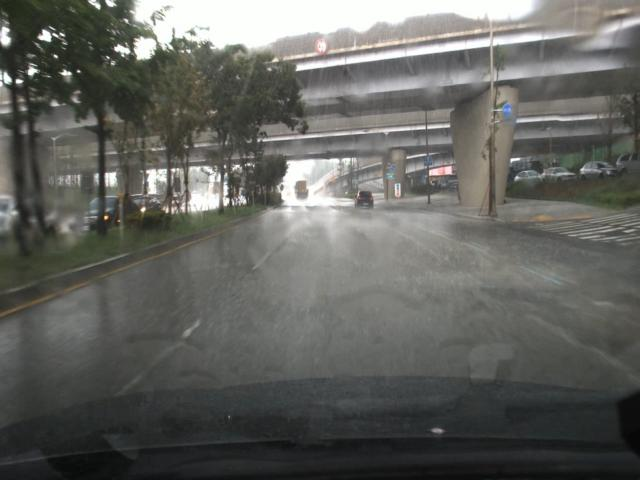
\includegraphics[width=2.7in, fbox]{Chapter5/scene_3-20160809_1425_34-000091.png}
        \caption{Blurred due to Wiper}
        \label{fig:blurbywiper}
    \end{subfigure}%
    ~
    \begin{subfigure}[b]{0.49\textwidth}
        \centering
        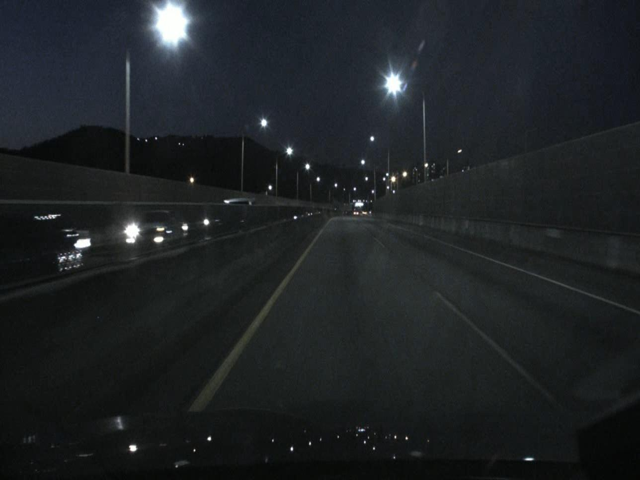
\includegraphics[width=2.7in, fbox]{Chapter5/scene_4-20160518_2015_42-000031.png}
        \caption{Low Luminance}
        \label{lowluminance}
    \end{subfigure}
    \\
    \begin{subfigure}[b]{0.98\textwidth}
        \centering
        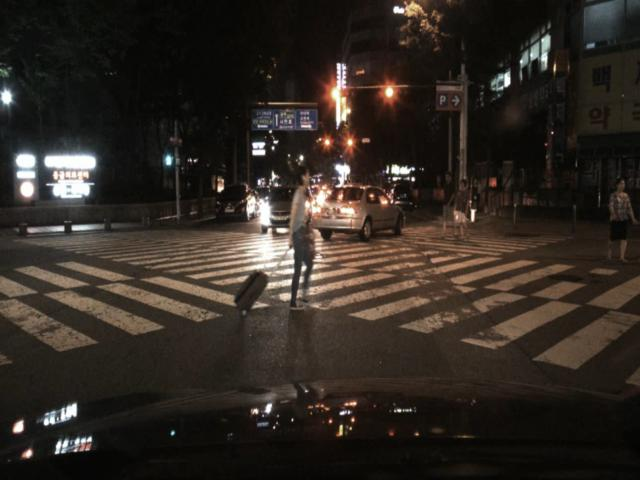
\includegraphics[width=2.7in, fbox]{Chapter5/scene_4-20160805_2122_57-000241.png}
        \caption{Complicated Situation}
        \label{fig:complicated}
    \end{subfigure}%
    \caption{Selected Images under Bad Weather Condition}
    \label{fig:rainyimg}
\end{figure}

\begin{enumerate}
    \item \texttt{scene\_2/20160510\_1302\_22/000181}, the serious reflection situation. As shown in \autoref{fig:heavylight}, the road is fuzzy by reflections. Thus the lane and the road end is not clear.
    \item \texttt{scene\_3/20160809\_1423\_33/000091}, the camera is blurred by heavy rain. As shown in \autoref{fig:blurbyrain}, rain drops blurred the sight, only outline of cars can be distinguished from background.
    \item \texttt{scene\_3/20160809\_1425\_34/000091}, the camera is blurred because the wiper has been just brushed on the glass, as shown in \autoref{fig:blurbywiper}.
    \item \texttt{scene\_4/20160518\_2015\_42/000031}, the light intensity is very low in dark night. As shown in \autoref{lowluminance}, the light source is only several street lamps in a very high place, and the entire scene is darksome. The lanes are blended into the background.
    \item \texttt{scene\_4/20160805\_2122\_57/000241}, crossroad in night with complicated road markings, pedestrian and heavy reflection, as shown in \autoref{fig:complicated}. There are too many interferent, which will distract or mislead the network.
\end{enumerate}

They are mainly selected from the scene $2 \sim 4$, because the scene $1$ don't have many images captured under rainy condition. The network performance on these pictures are given in $F_1$ score in \autoref{tab:rainyf1}. The first row is picture name, the second and third row is the per-class $F_1$ score (left to right, up to down is $1-17$ classes in \autoref{tab:classes}), and the fourth row is the average $F_1$ score for multi-classes.


\section{Selection of Confidential Threshold}
\label{sec:EX_threshold}

\begin{figure}[!ht]
    \centering
    \begin{subfigure}[b]{0.49\textwidth}
        \centering
        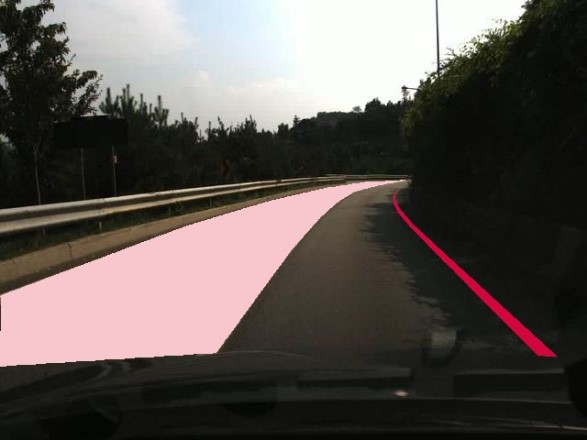
\includegraphics[width=2.7in, fbox]{Chapter5/Picture3an.jpg}
        \caption{Ground Truth}
    \end{subfigure}%
    ~
    \begin{subfigure}[b]{0.49\textwidth}
        \centering
        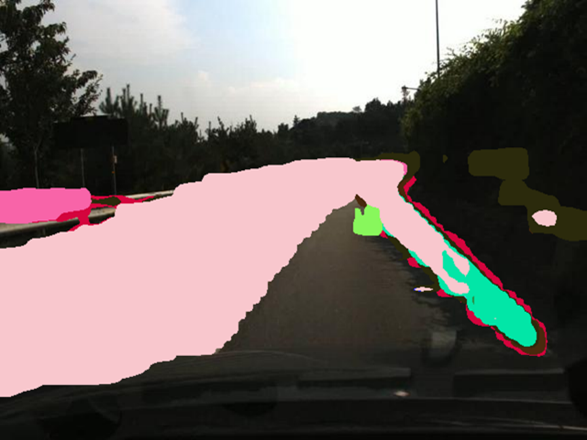
\includegraphics[width=2.7in, fbox]{Chapter5/pic1conf0.png}
        \caption{$\theta = 0.0\%$}
    \end{subfigure}
    \\
    \begin{subfigure}[b]{0.49\textwidth}
        \centering
        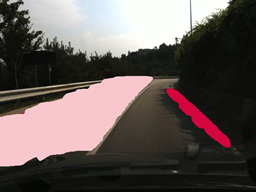
\includegraphics[width=2.7in, fbox]{Chapter5/pic1conf31.png}
        \caption{$\theta = 31.37\%$}
    \end{subfigure}%
    ~
    \begin{subfigure}[b]{0.49\textwidth}
        \centering
        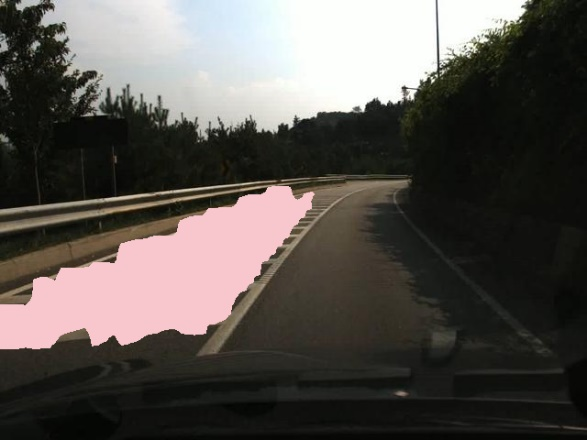
\includegraphics[width=2.7in, fbox]{Chapter5/pic1conf99.png}
        \caption{$\theta = 94.11\%$}
    \end{subfigure}
    \caption{Different Confidential Value for Sample 1}
    \label{fig:threshold1}
\end{figure}


The output of multi-label classification is a pixel-level confidential map. It will give a confidential value $C_i \in [0,100\%]$ for each pixel in each class. If the confidential value $C_{(x,y,c)}$ of certain pixel $(x,y)$ belonging to certain class $c$ is higher then threshold $\theta$, it is taken as $1$. Otherwise, it is taken as $0$, as shown in \autoref{eq:confidential}. Confidential threshold $\theta$ can be set manually. Higher $\theta$ will make the pixel label more confidential but may limit the network's imagination, while lower $\theta$ may make the image full of un-related classes, as shown in \autoref{fig:threshold1} and \autoref{fig:threshold2}.

\begin{equation}
\label{eq:confidential}
    f(C_{(x,y,c)})= 
    \begin{dcases}
        1, & \text{if } C_{(x,y)} \geq \theta\\
        0, & \text{otherwise}
    \end{dcases},\; \theta \in (0,1) 
\end{equation}

\begin{figure}[!ht]
    \centering
    \begin{subfigure}[b]{0.49\textwidth}
        \centering
        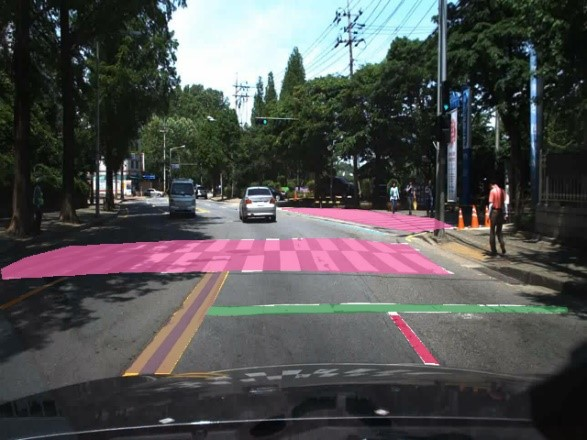
\includegraphics[width=2.7in, fbox]{Chapter5/Picture1an.jpg}
        \caption{Ground Truth}
    \end{subfigure}%
    ~
    \begin{subfigure}[b]{0.49\textwidth}
        \centering
        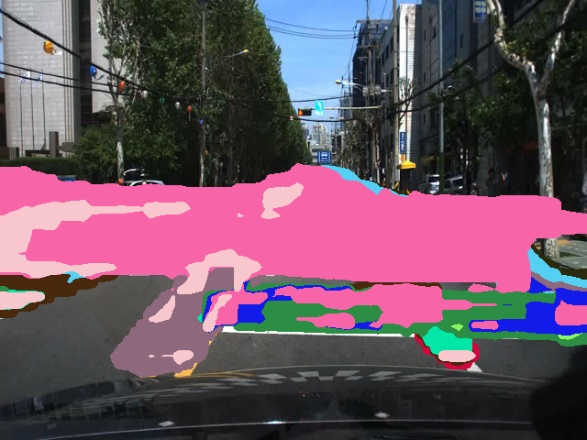
\includegraphics[width=2.7in, fbox]{Chapter5/pic2con0.png}
        \caption{$\theta = 0.0\%$}
    \end{subfigure}
    \\
    \begin{subfigure}[b]{0.49\textwidth}
        \centering
        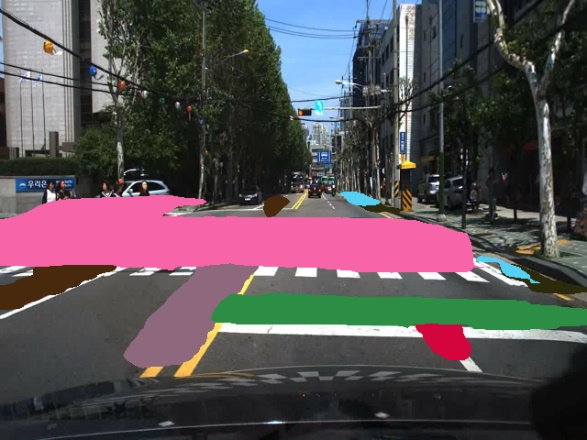
\includegraphics[width=2.7in, fbox]{Chapter5/pic2con23.png}
        \caption{$\theta = 23.52\%$}
    \end{subfigure}%
    ~
    \begin{subfigure}[b]{0.49\textwidth}
        \centering
        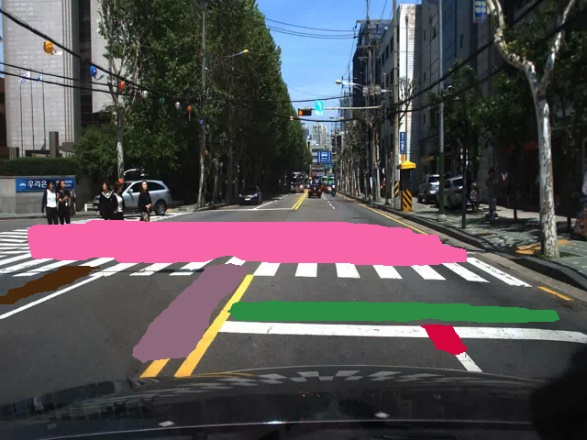
\includegraphics[width=2.7in, fbox]{Chapter5/pic2con70.png}
        \caption{$\theta = 70.59\%$}
    \end{subfigure}
    \caption{Different Confidential Value for Sample 2}
    \label{fig:threshold2}
\end{figure}

A recommended value based on empirical data is $\theta \in (20,30)$.

\section{Concluding Remarks}

This section discussed the experimental results of RVPGNet and especially talked about bad-weather condition. The network can achieve as high as $97.19\%$ accuracy and achieve the highest $99.73\%$ $F_1$ score under bad weather condition.

The next section will give a conclusion of this dissertation's work and its highlights. Also, it will explain some disadvantages in this dissertation and offer some directions for further research.

%=== END OF CHAPTER FIVE ===
\end{spacing}
\newpage
